\documentclass[]{article}
\usepackage[a4paper, total={15cm,23cm}]{geometry}
\usepackage{fancyhdr}
\usepackage{graphicx}
\usepackage{amsmath}
\usepackage{amssymb}
\usepackage{xcolor}
\usepackage{tikz}
\usepackage{verbatim}
\usepackage{tcolorbox}
\usepackage{textcomp}
\usepackage{xcomment}
%opening
\title{PH 223 Week 5}
\author{Benjamin Bauml}
\date{Winter 2024}
\pagestyle{fancy}
\rhead{PH 223}
\chead{Winter 2024}
\lhead{Week 5}

% For Assignment, leave Purpose as 0. For Worksheet, set to 1. For Student Solution, set to 2. For Teacher Solution, set to 3.
\newcommand{\Purpose}{0}

\newcommand{\Exclusion}{0}
\newcommand{\PageTurn}{0}
\newcommand{\GrayProb}{0}
\newcommand{\Tipsy}{0}

% Assignment
\if\Purpose0
\renewcommand{\Exclusion}{1}
\fi
% Worksheet
\if\Purpose1
\renewcommand{\Exclusion}{1}
\renewcommand{\PageTurn}{1}
\fi
% Student Solution
\if\Purpose2
\renewcommand{\PageTurn}{1}
\renewcommand{\GrayProb}{1}
\fi
% Teaching Copy
\if\Purpose3
\renewcommand{\PageTurn}{1}
\renewcommand{\GrayProb}{1}
\renewcommand{\Tipsy}{1}
\fi

\if\Exclusion1
\xcomment{Title,Problem,ProblemSub,PassFig}
\fi

\def \NewQ {0}
\def \PForce {0}
\newcommand{\MaybePage}[1]{
	\def \PForce {#1}
	\if\PForce1
		\newpage
	\else
		\if\NewQ0
		\gdef \NewQ {\PageTurn}
		\else
		\newpage
		\fi
	\fi
}

\newenvironment{Problem}[2][0]{%The first argument is optional, and if it is set to 1, the \newpage will be forced.
\MaybePage{#1}
\section*{#2}
\if\GrayProb1
\begin{tcolorbox}[colback=lightgray,colframe=lightgray,sharp corners,boxsep=1pt,left=0pt,right=0pt,top=0pt,bottom=0pt,after skip=2pt]
\else
\begin{tcolorbox}[colback=white,colframe=white,sharp corners,boxsep=1pt,left=0pt,right=0pt,top=0pt,bottom=0pt,after skip=2pt]
\fi
}{
\end{tcolorbox}\noindent
}

\newenvironment{ProblemSub}[1][0]{%The argument is optional, and if it is set to 1, a \newpage will be forced.
	\def \PForce {#1}
	\if\PForce1
	\newpage
	\fi
\if\GrayProb1
\begin{tcolorbox}[colback=lightgray,colframe=lightgray,sharp corners,boxsep=1pt,left=0pt,right=0pt,top=0pt,bottom=0pt,after skip=2pt]
\else
\begin{tcolorbox}[colback=white,colframe=white,sharp corners,boxsep=1pt,left=0pt,right=0pt,top=0pt,bottom=0pt,after skip=2pt]
\fi
}{
\end{tcolorbox}\noindent
}

\newenvironment{PassFig}{\begin{figure}[h]}{\end{figure}}

\newcommand{\TeachingTips}[1]{
\if\Tipsy1
\begin{tcolorbox}[colback=lightgray,colframe=black]
#1
\end{tcolorbox}
\fi
}

\newenvironment{Title}{\maketitle}{}

\begin{document}
\begin{Title}
\begin{center}
	These problems are borrowed/adapted from Chapter 28 of the \textit{Student Workbook} for \textit{Physics for Scientists and Engineers}.
\end{center}
\end{Title}

\begin{Problem}{Activity 1}
	Rank in order, from largest to smallest, the three currents $ I_{1} $ to $ I_{3} $.
\end{Problem}
\begin{PassFig}
	\centering
	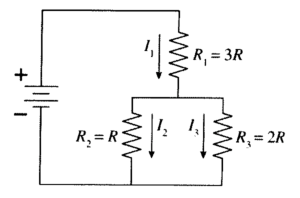
\includegraphics[scale=1]{A2a}
\end{PassFig}

\noindent Order: $ I_{1} > I_{2} > I_{3} $ \\
Explanation: By Kirchhoff's junction rule, $ I_{1} = I_{2} + I_{3} $, so $ I_{1} $ must be larger than both of the other two currents. The voltage drop across $ R_{2} $ and $ R_{3} $ is the same, but $ R_{2} < R_{3} $, so $ I = \frac{\Delta V}{R} $ suggests that $ I_{2} > I_{3} $.

\begin{Problem}{Activity 2}
	(a) Consider the points $ a $ and $ b $. Is the potential difference $ \Delta V_{ab} = 0 $? If so, why? If not, which point is more positive?
\end{Problem}
\begin{PassFig}
	\centering
	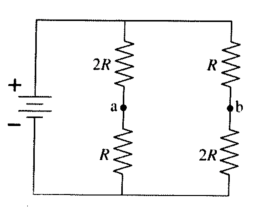
\includegraphics[scale=0.9]{A2b}
\end{PassFig}

\noindent No, the potential difference is not zero. Each branch of the circuit has the same effective resistance and the same voltage drop, so by $ \Delta V = I R $, we know $ I_{a} = I_{b} $. However, this also suggests that the voltage drop across the $ 2R $ resistor is greater than the voltage drop across the smaller resistor. As such, point $ b $ is more positive.
\begin{ProblemSub}
	(b) If a wire is connected between points $ a $ and $ b $, does a current flow through it? If so, in which direction---to the right or to the left? Explain.
\end{ProblemSub}
Current flows to the left from $ b $ to $ a $. The connecting wire will cause $ a $ and $ b $ to be at equal potentials. Now, the current across the first pair of parallel resistors will favor the path of least resistance. Since $ \Delta V $ from the top of the circuit to the $ a $ and $ b $ connection is the same for both resistors, but one has twice the resistance, the $ 2R $ resistor will have half as much current as the $ R $ resistor. The same goes for the lower pair of resistors. Half of the current leaving the top $ R $ resistor will cross from $ b $ to $ a $ to enter the bottom $ R $ resistor.

\begin{Problem}[1]{Activity 3}
	The graph shows the voltage as a function of time on a capacitor as it is discharged (separately) through three different resistors. Rank in order, from largest to smallest, the values of the resistances $ R_{1} $ to $ R_{3} $.
\end{Problem}
\begin{PassFig}
	\centering
	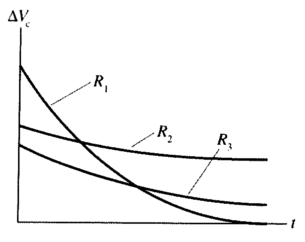
\includegraphics[scale=1]{A3}
\end{PassFig}

\noindent Order: $ R_{2} > R_{3} > R_{1} $ \\
Explanation: The decay time of an RC circuit is $ \tau = RC $. The decay time is longest for the $ R_{2} $ curve and shortest for the $ R_{1} $ curve. Since they all share the same capacitor, this directly corresponds to their relative resistances.

\TeachingTips{
For a discharging capacitor, the loop law is
\[
0 = -V_{C} - V_{R} = -\frac{Q}{C} - IR = -\frac{Q}{C} - \frac{dQ}{dt}R,
\]
which may seem strange, since it assumes that current goes into the positive end of the capacitor (thus allowing both voltage changes to be negative as we go with the current through the resistor and then from the positive terminal of the capacitor to its negative terminal). After all, we know the current should be going the other way. However, if we make that change, then we must redefine the current to be $I = -\frac{dQ}{dt}$, since a positive current flowing away from the capacitor would reduce the charge on it. Either way, the differential equation is
\[
\frac{dQ}{dt} = -\frac{Q}{RC},
\]
and the solution is
\[
Q(t) = Q_{0}e^{-t/RC}.
\]
When we take the derivative, we find that
\[
I(t) = -\frac{Q_{0}}{RC}e^{-t/RC},
\]
and we see that the current is going the opposite direction from what we assumed! That said, this problem deals with the voltage:
\[
V_{C}(t) = \frac{Q(t)}{C} = \frac{Q_{0}}{C}e^{-t/RC}.
\]
}
\TeachingTips{
The solution for a charging capacitor (see the next activity) is $Q(t) = C\Delta V_{bat}\left(1-e^{-t/RC}\right)$, which differentiates to $I(t) = \frac{\Delta V_{bat}}{R}e^{-t/RC}$.
}

\begin{Problem}{Activity 4}
	The charge on the capacitor is zero when the switch closes at $ t = 0 $ s.
\end{Problem}
\begin{PassFig}
	\centering
	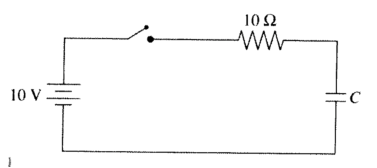
\includegraphics[scale=1]{A4}
\end{PassFig}
\begin{ProblemSub}
	(a) What will be the current in the circuit after the switch has been closed for a long time? Explain.
\end{ProblemSub}
After the switch has been closed a long time, the capacitor will be fully charged and the current will approach zero.
\begin{ProblemSub}
	(b) Immediately after the switch closes, before the capacitor has had time to charge, the potential difference across the capacitor is zero. What must be the potential difference across the resistor in order to satisfy Kirchhoff's loop law? Explain.
\end{ProblemSub}
Going clockwise, Kirchhoff's loop law gives
\[
0 = \Delta V_{bat} + \Delta V_{R} + \Delta V_{C}.
\]
We know that $ \Delta V_{bat} = \mathcal{E} = 10 $ V. $ \Delta V_{C} = -Q/C $, but the capacitor hasn't charged, so this is zero. As such
\[
0 = \mathcal{E} + \Delta V_{R},
\]
so $ \Delta V_{R} = -10 $ V.
\begin{ProblemSub}
	(c) Based on your answer to part (b), what is the current in the circuit immediately after the switch closes?
\end{ProblemSub}
The current in the circuit is the same as the current through the resistor, and by Ohm's law (using $ \Delta V_{R} = 10 $ V, the magnitude of the potential difference, to remove the sign issue), we know that
\[
I = \frac{\Delta V_{R}}{R} = \frac{10\text{ V}}{10\text{ \textohm}} = 1\text{ A}.
\]
\begin{ProblemSub}
	(d) Sketch a graph of the current versus time, starting from just before $ t = 0 $ s and continuing until the switch has been closed for a long time. There are no numerical values for the horizontal axis, so you should think about the \textit{shape} of the graph.
\end{ProblemSub}
The current decays as charge accumulates on the capacitor and its voltage drop $ \Delta V_{C} $ increases. $ \Delta V_{bat} $ is constant, so $ \Delta V_{R} $ must decrease as $ \Delta V_{C} $ increases.
\begin{PassFig}
	\centering
	\if\GrayProb0
		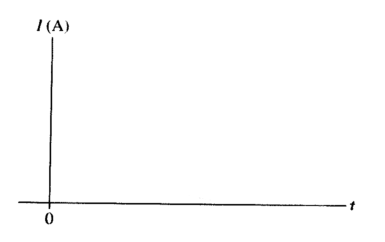
\includegraphics[scale=1]{A4d}
	\else
		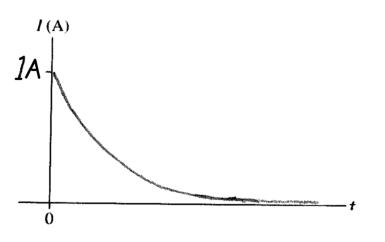
\includegraphics[scale=1]{A4dSol}
	\fi
\end{PassFig}
\end{document}
